%%
%% This is file `tikzposter-template.tex',
%% generated with the docstrip utility.
%%
%% The original source files were:
%%
%% tikzposter.dtx  (with options: `tikzposter-template.tex')
%% 
%% This is a generated file.
%% 
%% Copyright (C) 2014 by Pascal Richter, Elena Botoeva, Richard Barnard, and Dirk Surmann
%% 
%% This file may be distributed and/or modified under the
%% conditions of the LaTeX Project Public License, either
%% version 2.0 of this license or (at your option) any later
%% version. The latest version of this license is in:
%% 
%% http://www.latex-project.org/lppl.txt
%% 
%% and version 2.0 or later is part of all distributions of
%% LaTeX version 2013/12/01 or later.
%% 




\documentclass[24pt]{tikzposter} %Options for format can be included here

 % Title, Author, Institute
\title{Towards Atomistic Stress Corrosion Cracking of Ti Alloys}
\author{Tigany Zarrouk}
\institute{King's College London}
\titlegraphic{../Images}

 %Choose Layout
\usetheme{Default}

\begin{document}

 % Title block with title, author, logo, etc.
\maketitle
\block{Introduction}{
  \begin{itemize}
     \item How does oxygen play a role in solution hardening in Ti alloys?\\
   \item Dislocations are defects that have an atomistic origin. They are line defects. \\
   \item How does atomic oxygen interfere with dislocations which in turn changes how  the plasticity of titanium as a whole?\\
   \item Screw dislocations are the most important as they have the least mobility in hcp.\\
   \end{itemize}
}
 \begin{columns}

 % FIRST column
\column{0.6}% Width set relative to text width

\block{Large Column}{Text\\Text\\Text Text Text}
\note{Note with default behavior}
\note[targetoffsetx=12cm, targetoffsety=-1cm, angle=20, rotate=25]
{Note \\ offset and rotated}

 % First column - second block
\block{Block titles with enough text will automatically obey spacing requirements }
{Text\\Text}

 % First column - third block
\block{Sample Block 4}{T\\E\\S\\T}

 % SECOND column
\column{0.4}
 %Second column with first block's top edge aligned with with previous column's top.

 % Second column - first block
\block[titleleft]{Smaller Column}{Test}

 % Second column - second block
\block[titlewidthscale=0.6, bodywidthscale=0.8]
{Variable width title}{Block with smaller width.}

 % Second column - third block
\block{}{Block with no title}

 % Second column - A collection of blocks in subcolumn environment.
\begin{subcolumns}
    \subcolumn{0.27} \block{1}{First block.} \block{2}{Second block}
    \subcolumn{0.4} \block{Sub-columns}{Sample subblocks\\Second subcolumn}
    \subcolumn{0.33} \block{4}{Fourth} \block{}{Final Subcolumn block}
\end{subcolumns}

 % Bottomblock
\block{Final Block in column}{
    Sample block.
}
\end{columns}
\begin{columns}
    \column{0.5}
    \block{A figure}
    {
        \begin{tikzfigure}
            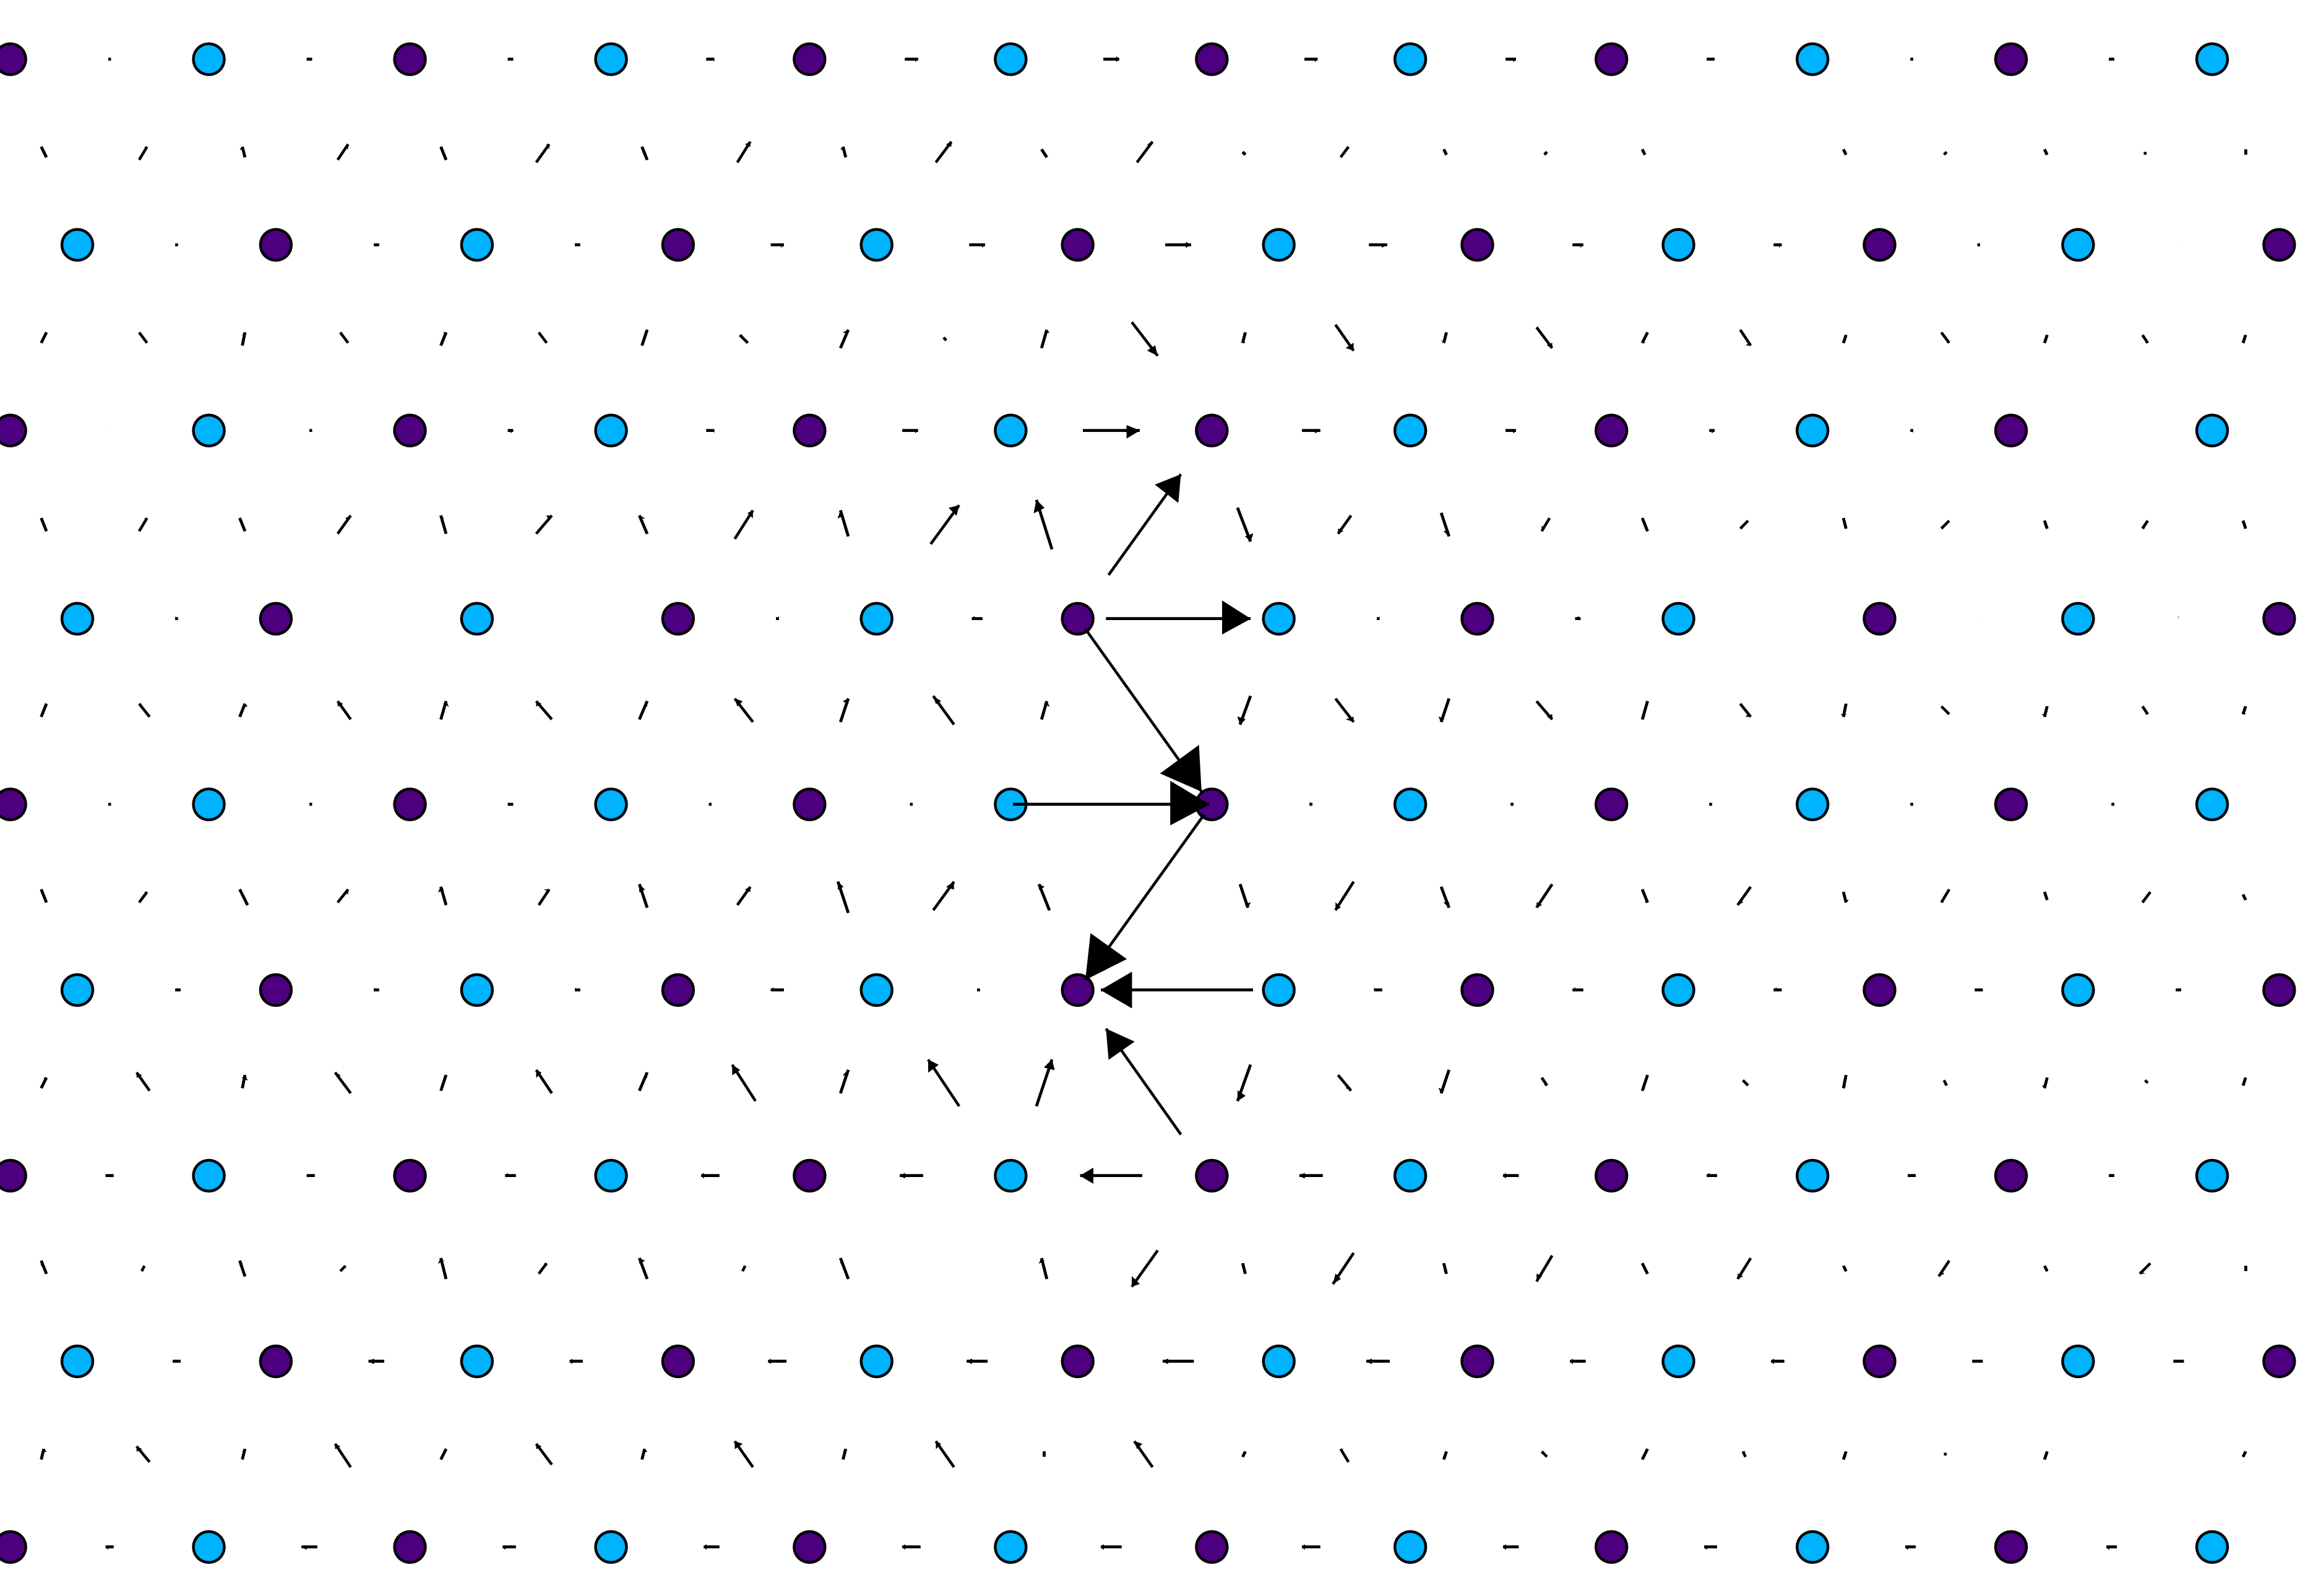
\includegraphics[width=0.4\textwidth]{../Images/zoom_core_look.png}
        \end{tikzfigure}
    }
    \column{0.5}
    
    \block{Relaxed core of a dislocation in an 'S' quadrupolar
    configuration.}{Relaxed core of this dislocation matches very well with
    literature. ***  See Ghazisaeidi and Trinkle  ***}
\end{columns}


\block[titleleft, titleoffsetx=2em, titleoffsety=1em, bodyoffsetx=2em,%
 bodyoffsety=-2cm, roundedcorners=10, linewidth=0mm, titlewidthscale=0.7,%
 bodywidthscale=0.9, bodyverticalshift=2cm, titleright]
{Block outside of Columns}{Along with several options enabled}

\end{document}



\endinput
%%
%% End of file `tikzposter-template.tex'.
